\section{Dimensionierung}
Dieses Kapitel stellt eine Zusammenstellung der ausgelegten Komponenten dar. Es wird beschrieben, wie die Komponenten ausleget, und welche Überlegungen bei der Auslegung gemacht wurden. Die Berechnungen wurden mit einer Excel-Tabelle getätigt, welche im elektronischen Anhang ANHANG einsehbar ist.

\subsection{Boden}
Der Fussboden des Solar Butteflys soll als Sandwichstruktur realisiert werden, wobei als Deckschicht Aluminiumblech und als Kern geschäumtes Ocean-PET verwendet werden soll. Der Fussboden muss die Personenlasten aufnehmen und auf das Chassis übertragen. Weiter sieht das zum Zeitpunkt der Durchführung dieser Arbeit verfolgte Konzept vor, dass die Seitenmodule während der Fahrt über den Boden mit dem Rest der Struktur verbunden und befestigt werden. Im Rande des Bodens sollen abschnittweise Aluminiumprofile eingebettet werden, an welchen die Seitenmodule befestigt werden können.\\
Zu Begin der Ausarbeitung des Konzeptes wurden umrahmende Aluminiumprofile aus dem Fahrzeugbau in betracht gezogen, welche auf Platten mit einer Dicke von 25mm passen. Eine erste Annahme der Dicke des Bodens wurde so getroffen, dass diese in die besagten Profilen passen. Über eine Absprache mit einem Experten aus dem Wohnmobilbau wurde in erfahrung gebracht, dass in Wohnmobilen häuffig Fussböden mit einer Dicke von 30 mm, mit einer Dicke der Deckschichten von 1 mm, verbaut werden. [QUELLE] Weiter wurde mitgeteilt, dass die erste Abschätzung der Dicke von 25 mm eine plausible sei.\\

Um die getroffene Abschätzung zu überprüfen und die Dicke der Deckschichten zu bestimmen, wurden für zwei Belastungsfälle berechnungen angestellt. Die Fallunterscheidung sowie die Idealisierungen der Lagerung und Krafteinleitung der beiden Fälle ist in der Abbildung \ref{Boden Idealisierung} dargestellt.

\begin{figure}[!ht]
  \centering
    \begin{subfigure}{.5\textwidth}
      \centering
      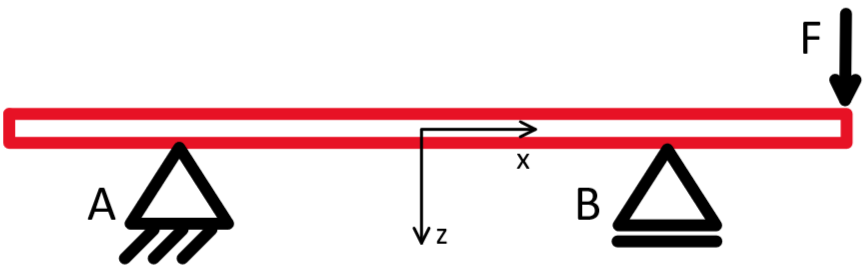
\includegraphics[width=.98\linewidth]{04_figures/Boden Fall1.png}
      \caption{Belastungsfall 1}
      \label{Belastungsfall 1}
    \end{subfigure}%
    \begin{subfigure}{.5\textwidth}
      \centering
      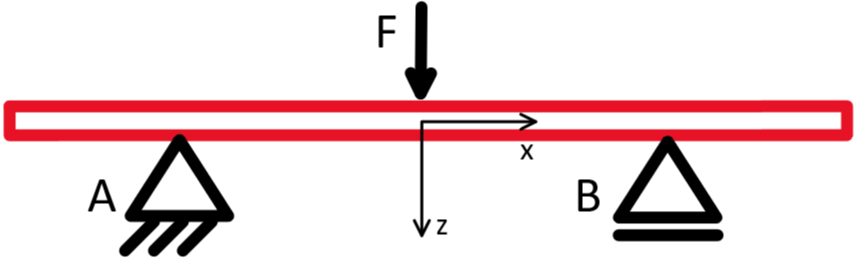
\includegraphics[width=.98\linewidth]{04_figures/Boden Fall2.png}
      \caption{Belastungsfall 2}
      \label{Belastungsfall 2}
    \end{subfigure}%
  \caption{Darstellung der beiden Belastungsfällen und deren Idealisierungen}
\label{Boden Idealisierung}
\end{figure}

Als Belastung wird eine Masse von 200 kg gewählt, welche auf einen 1000 mm langen Bodenabschnitt eingeleitet wird. Der Boden hat eine Breite von 2050 mm und der Abstand zwischen den Lagern beträgt 1410 mm. In der Abbildung \ref{Boden QM} sind die Querkraft- und Biegemomentenverläufe der beiden Fälle dargestellt.

\begin{figure}[!ht]
  \centering
    \begin{subfigure}{.5\textwidth}
      \centering
      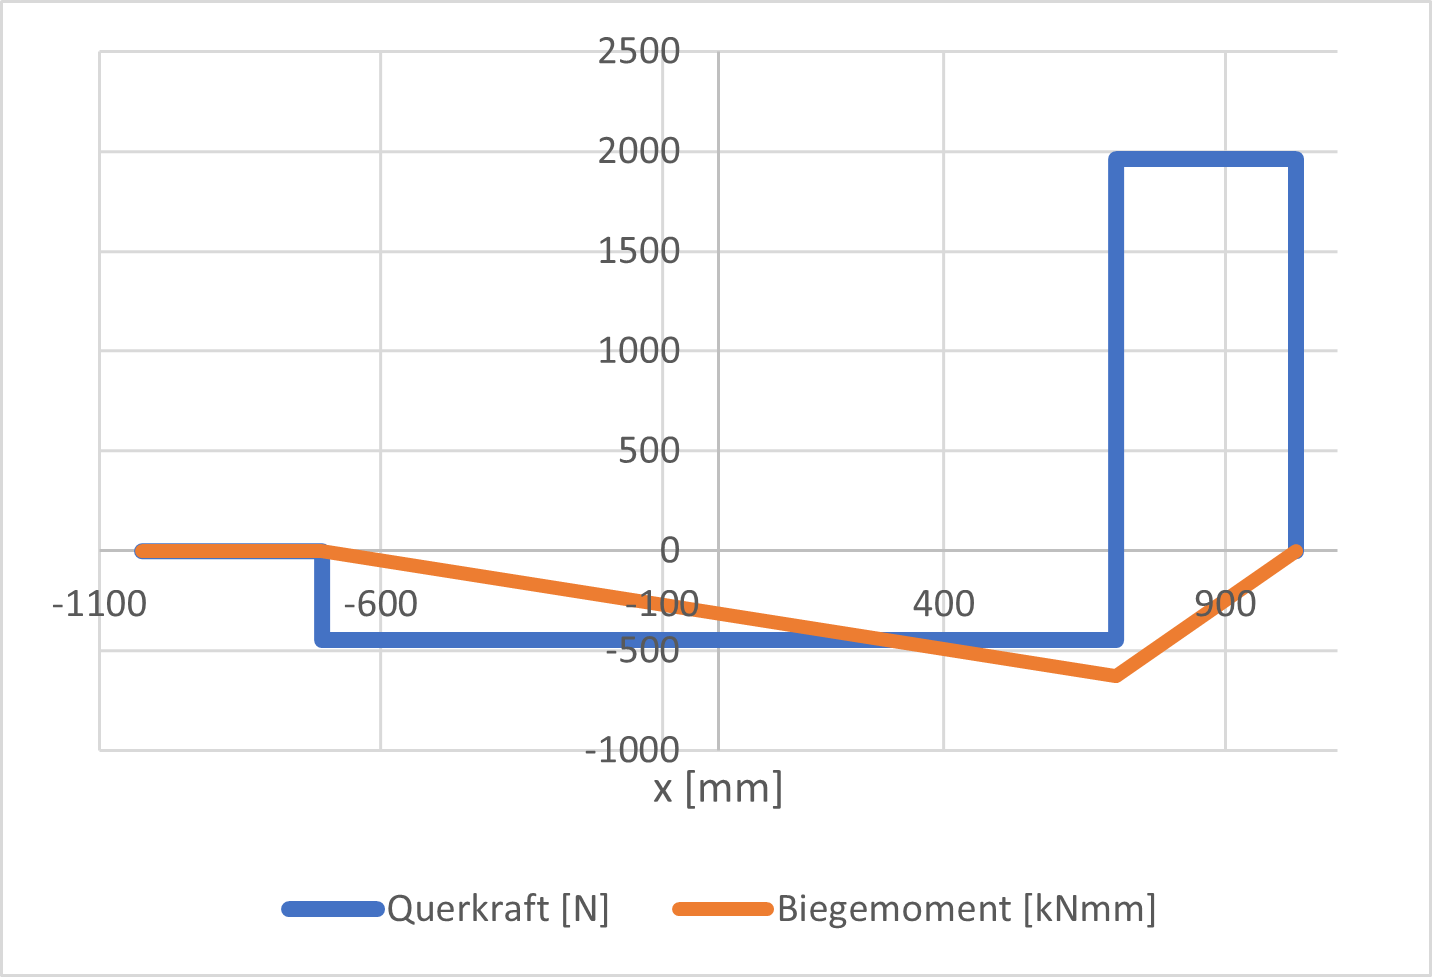
\includegraphics[width=.98\linewidth]{04_figures/Boden QM1.png}
      \caption{Belastungsfall 1}
      \label{Belastungsfall 1}
    \end{subfigure}%
    \begin{subfigure}{.5\textwidth}
      \centering
      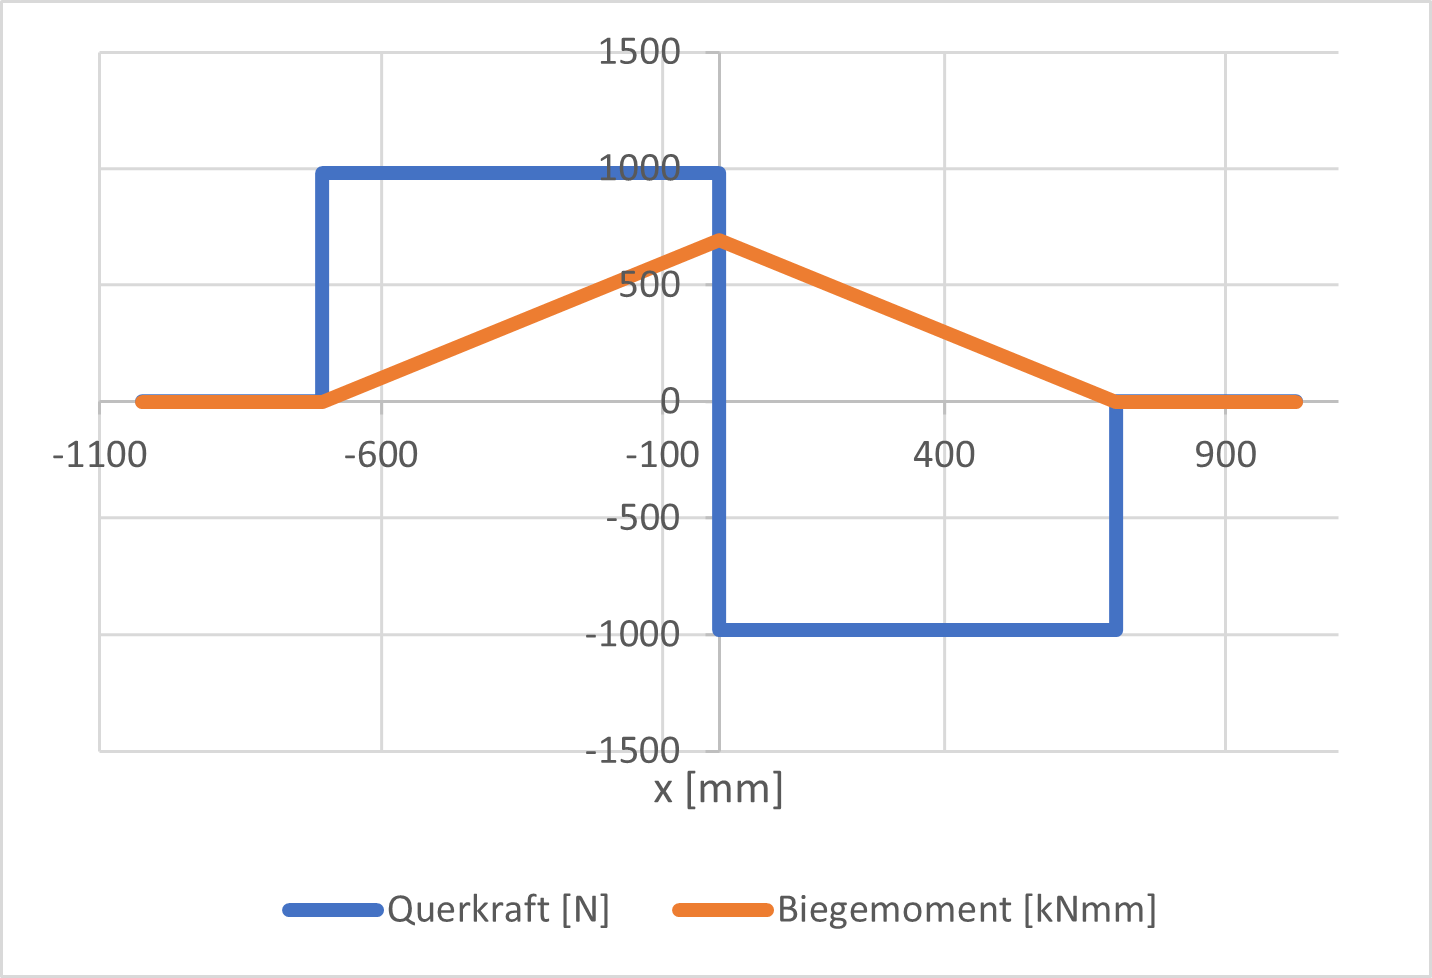
\includegraphics[width=.98\linewidth]{04_figures/Boden QM2.png}
      \caption{Belastungsfall 2}
      \label{Belastungsfall 2}
    \end{subfigure}%
  \caption{Querkraft- und Biegemomentenverläufe der Bodenplatten}
\label{Boden QB}
\end{figure}

Deckschicht von 0.36 mm spannung von 80 MPa. 

Schubbeulen und Knittern!


Missbrauchslastfälle: Spitzer Schuh, Druckbelastung, Dellen,
Empfehlung: 1mm Gwicht: Viel Potential, Risiko in kauf nehmen, Falls schaden: einfach zu reparieren.




\subsection{Dach - Hauptmodul}
Beschreibung:
  Aluminiumprofile: Tragen der Panelen
  Unterbringung der Verschlüsse

  \paragraph{Berechnung}\mbox{}//
    Limitierender Faktor: Deformation
    Berücksichtigung des Eigengewichtes,
    Mittragende Breite des Daches


\subsection{Panelen}
  Erste Berechnung wie Dach, dann jedoch schwierig wegen komplexer aufhängung und 2D-Problem.
  Darum FEM:
    Eigengewicht, Beschleunigung, Extra Last mit Druck.

  Einfache Lagerung: Resultate stimmen überein mit Excel.
  Neue Aufhängungen:
    Verformungen und Bilder.
    Schluss in der Arbeit von BACHER.
